\documentclass[sigconf,nonacm]{acmart}

% meta-data -- adjust to meaningful values
\title{Project Report -- Group 12}
\author{Kris van Melis, Nicolae Rusnac, Reinout Vos, Bram de Vries}

% remove overhead that is used in regular ACM papers
\settopmatter{printacmref=false} % box after abstract
\renewcommand\footnotetextcopyrightpermission[1]{} % copyright on first page
\pagestyle{plain} % running headers

\usepackage[utf8]{inputenc}
\usepackage[T1]{fontenc}
\usepackage{xcolor}

\begin{document}

\begin{abstract}
% !TEX root =  ../report.tex
TODO
\end{abstract}

\maketitle

% IMPORTANT: Report Knock-out Criteria:
% • The report follows the formatting guidelines.
% • The report follows the expected structure.
% • The report contains elaborated text and balances the content between the different parts.
% • The language quality is high and it is easy to read and follow the report.

% Each section has a corresponding file in the 'contents' folder
% !TEX root =  ../report.tex
\section{Introduction}
First things first, we started this project with a {\color{blue}\href{https://www.kaggle.com/code/luiscruz/phishing-detection-cnn?scriptVersionId=173193829}{Machine Learning model}} for detecting URL phishing, which is the act of fraudulently manipulating victims to click on links in order to obtain their credentials, banking information, or passwords. Our goal is to design an application around this model and deploy it, such that the application is production-ready. 
Therefore, in this document you will be able to find the overall setup of the project, with the corresponding design decisions we took in order to realize our goal. A link to our GitHub organization can be found here:
{\color{blue} \url{https://github.com/remla24-team12}}.

\subsection{Use Cases}
The use cases of the application are fairly straightforward: \\
Firstly, the user can provide a URL of their choice as input, then the model makes a prediction whether the URL is valid or phishing, finally the prediction is displayed to the user. \\
Afterwards, the user is asked to give feedback on the prediction. This will help improve the accuracy of the model over time: If the users deems the prediction to be incorrect, we can either update the label for the URL, or when the URL is not yet present in the dataset, we obtain a new entry with a human-verified label. 

\subsection{Architecture}
When designing the application we decided to stick to the architecture proposed in the assignment, see fig. {\color{red}\ref{fig:architecture}}.
For this micro-services architecture all components are built independently and interact with each other through package dependencies or APIs. \\
Every component is developed its own corresponding repository (except \texttt{app-frontend} and \texttt{app-service}, which are combined into one). Additionally, we use a \texttt{provisioning} repository which acts as the central repository containing all information about running the application and operating the cluster.
Regarding the purpose of the other components, we have the app:
\begin{itemize}
    \item \texttt{app-frontend} : Receives input from the user and forwards this to the \texttt{app-service} using an API.
    \item \texttt{app-service} : Middle man between frontend and backend, queries the \texttt{model-service} using an API and forwards this to the frontend.
    \item \texttt{lib-version} : Library containing version of the app, used for automatic versioning.
\end{itemize}

And the model:
\begin{itemize}
    \item \texttt{model-training} : Trains the model and stores it publicly such that the \texttt{model-service} can access it.
    \item \texttt{model-service} : Acts as a wrapper for the released model through an API. Receives request from \texttt{app-service}, queries the model and sends the response back.
    \item \texttt{lib-ml} : Contains pre-processing logic for data that is used for training or queries.
\end{itemize}

\begin{figure*}
    \centering
    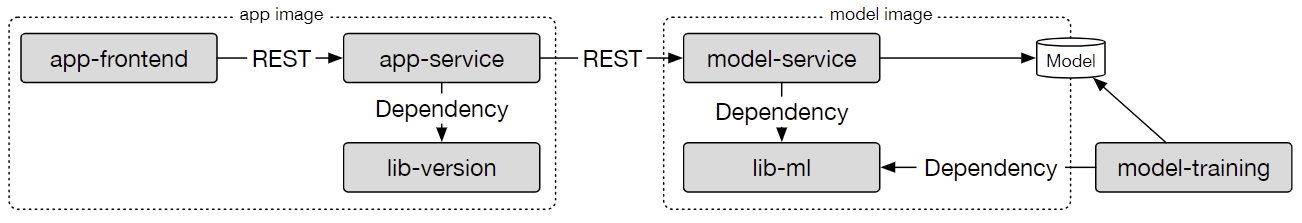
\includegraphics[width=1\linewidth]{images/architecture.png}
    \caption{Application Architecture}
    \label{fig:architecture}
\end{figure*}


% • Name the different pipeline steps.
% • Elaborate their purpose and implementation, including the used tools.
% • Discuss the data flow throughout the steps and name the relevant artifacts/data.
% A new team member should be able to understand your release processes and where the artifacts get published.

% Insufficient -> At least one of the pipelines is not documented.
% Sufficient -> Two pipeline for release a package and an image are described. All pipeline steps get introduced.
% Good -> The report describes the purpose of all pipeline steps and introduces the relevant tools. The documentation visualizes the pipelines and connects the text.
% Very Good -> The documentation introduces relevant artifacts/data and their dependencies/flow.
% Excellent -> The documentation makes it easy for new team members to get started with contributing to the project. It becomes easy to understand the build pipelines, e.g., how models and releases are built and where artifacts get published.
\section{Release Pipelines}
Because we adopt the micro-services architecture, instead of releasing the entire application in one single package, each individual component is released separately. This process of releasing varies depending on the type of component. Therefore, in order to automate these configurations we make use of {\color{blue} \href{https://docs.github.com/en/actions/using-workflows}{GitHub Actions}}, i.e. workflows.

\subsection{Software Package}
The first type of workflow is configured for a software package. During this process a repository is built, after which the artifact is stored in a package repository. For example, the workflow for \texttt{lib-version} publishes the library to {\color{blue} \href{https://github.com/features/packages}{GitHub Packages}}. Fig. {\color{red} \ref{fig:libversion-workflow}} shows a visualization of this process.

\subsubsection{Automatic Versioning}
Before releasing the package it is important that we update its version. For this we define another {\color{blue}\href{https://github.com/remla24-team12/lib-version/blob/main/.github/workflows/version.yml}{workflow}}, which is triggered by pushes directly to the main branch (which is a bad practice, but its included to be safe) or by pull requests to the main branch. The version itself is defined using a Git tag. The stages of this workflows are as follows:
\begin{itemize}
    \item \textbf{Increment version}: This stage looks up the latest tag and bumps it up. Currently, we always increment the patch for simplicity, meaning minor and major releases are not supported. This is a future improvement.
    \item \textbf{Create Git tag}: Once the new tag number has been computed, a new tag is created and pushed. 
\end{itemize}

The {\color{blue}\href{https://github.com/remla24-team12/lib-version/blob/main/.github/workflows/release.yml}{release workflow}} is triggered after the automatic versioning workflow has been completed.
Afterwards the following stages are executed:
\begin{itemize}
    \item \textbf{Get latest tag}: Retrieve the tag created in the versioning workflow.
    \item \textbf{Set up Node.js}: Configure Node.js environment to use GitHub Packages as the registry and set the appropriate scope.
    \item \textbf{Install dependencies}: Install necessary node packages as defined in package.json.
    \item \textbf{Update version}: Update the package.json file with the version from the latest git tag.
    \item \textbf{Build and publish package}: Builds the npm package and publishes it to GitHub Packages using the authentication token provided through a secret.
\end{itemize}

\begin{figure*}
    \centering
    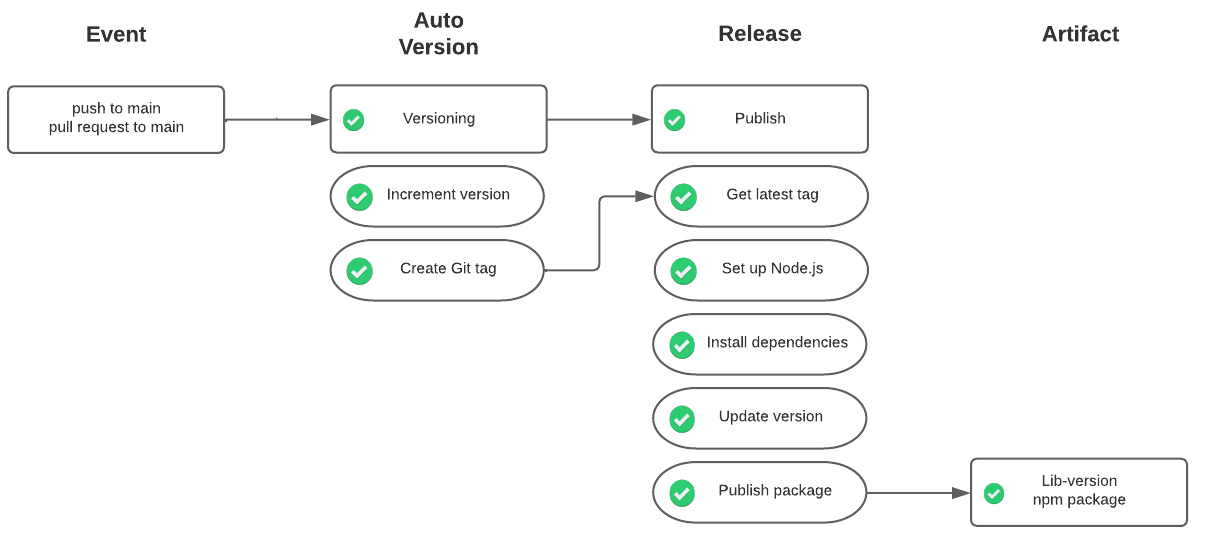
\includegraphics[width=0.75\linewidth]{images/libversion_workflow.png}
    \caption{Visualization of \texttt{lib-version} workflows}
    \label{fig:libversion-workflow}
\end{figure*}
% Visualization tool: 
% https://lucid.app/lucidchart/38c9ce70-2d27-459d-b58a-c52e3883af58/edit?beaconFlowId=119EFCC8C64C2A8A&invitationId=inv_871bb54d-8a09-4c35-afbd-f00ea69222e8&page=0_0#

\subsection{Container Image}
The release of container images is similar across the different services in our application with some variation in cases where we require secretes to access parts of it. We have three images that we use in our deployment: \emph{model-service}, \emph{app-frontend} and \emph{app-backend}. The general workflow for the images is:
\begin{itemize}
    \item \textbf{Fetch secrets}: Fetch GitHub stored as files from the release workflow
    \item \textbf{Copy app files}: Copy all the files of the application alongside the secrets.
    \item \textbf{Install dependencies}: Install the dependencies using either npm or pipenv.
    \item \textbf{Expose ports}: Expose the ports on which the applications run.
    \item \textbf{Run the application}: Run the command to start the applications.
\end{itemize}
We only need to copy secrets for \emph{app-frontend} and \emph{model-service}. In the case of \emph{frontend} we need an authentication token to use in the .npmrc file in order to be able to use the library. In the case of \emph{model-service} we need to use login credentials to the google drive where we host our dvc pipeline data, since we are using the DVC live library to fetch the machine learning model. The current way of handling secrets is not secure, since one could simply enter the docker file and take a look at the secret files. For the scope of the project, we consider this to be enough. The general release workflow of the images is similar to the lib-version and looks like this:
\begin{itemize}
    \item \textbf{Get latest tag}: Retrieve the tag created in the versioning workflow.
    \item \textbf{Write secrets to file}: Write the secrets from GitHub secret environment variables to files.
    \item \textbf{Log in to GitHub Container Registry}: Provide the token for login
    \item \textbf{Build and publish package}: Builds the docker image and publishes it to GitHub Packages using the authentication token provided through a secret and the newly updated version which was bumped.
\end{itemize}
% Document the final deployment of your application.
% • Visualize the structure of the deployment (the entities and their connections).
% • The diagram should illustrate the data flow for incoming requests.
% • Include all resources that you have deployed in the cluster and their connections (not just the ones that are relevant for serving requests).
% • Clarify the visualization through a concise elaboration.

% Insufficient -> The deployment documentation is incomprehensible or incomplete.
% Sufficient -> The deployment documentation is limited to the structure of the deployment (the entities and their connections) or the data flow for incoming requests. The documentation visualizes the deployment and connects the text.
% Good -> The deployment documentation describes both the structure of the deployment (the entities and their connections) and the data flow for incoming requests.
% Very Good -> The deployment documentation includes all deployed resource types and relations.
% Excellent -> The deployment documentation is visually appealing and clear. It is easy for a new team member to understand and to start contributing to the described system.

% Interesting visualization tool:
% https://diagrams.mingrammer.com/docs/getting-started/examples

\section{Deployment}
We host our application on a set of virtual machine (VM) nodes. This is achieved using {\color{blue} \href{https://www.vagrantup.com/}{Vagrant}} and {\color{blue} \href{https://www.ansible.com/}{Ansible}}. Vagrant is a tool used to create and manage VM environments in a single workflow. Then, Ansible is an automation tool for provisioning, configuring, and managing the VMs.

The actual provisioning and deployment is done using {{\color{blue} \href{https://kubernetes.io/}{Kubernetes}}}.
Our deployment consists of multiple services and deployments managed within a Kubernetes cluster, utilizing {\color{blue} \href{https://istio.io/}{Istio}} for advanced traffic management. See figure {\color{red} \ref{fig:k8s_istio}}. The core components include frontend and backend services, along with a model service.

The app-frontend service has two versions of deployments (app-frontend-v1 and app-frontend-v2), each running with one replica. The app-service and model-service are also deployed with a single replica each, exposing ports 3000 and 5000, respectively.

We use Istio to manage the ingress traffic through the app-gateway, which is configured to listen on port 80 for HTTP traffic. The app-virtualservice directs traffic to different services based on the URI path. Requests with the prefix '/app' are routed to the app-frontend service, with 80\% of the traffic directed to version 1 and 20\% to version 2. Requests to '/api' are routed to the app-service on port 3000, and requests to '/model' are routed to the model-service on port 5000. Additionally, installed using {\color{blue} \href{https://helm.sh/}{Helm}}, we use monitoring tools like {\color{blue}\href{https://prometheus.io/docs/introduction/overview/}{Prometheus}} and {\color{blue} \href{https://duckduckgo.com/?q=grafana&ia=web}{Grafana}} to collect and monitor metrics. The corresponding '/metrics' and '/grafana' paths are directed to   services for monitoring and visualization purposes. 

This setup allows for robust service management, version control, and traffic routing, ensuring high availability and scalability of our application.


\begin{figure}[h]
    \centering
    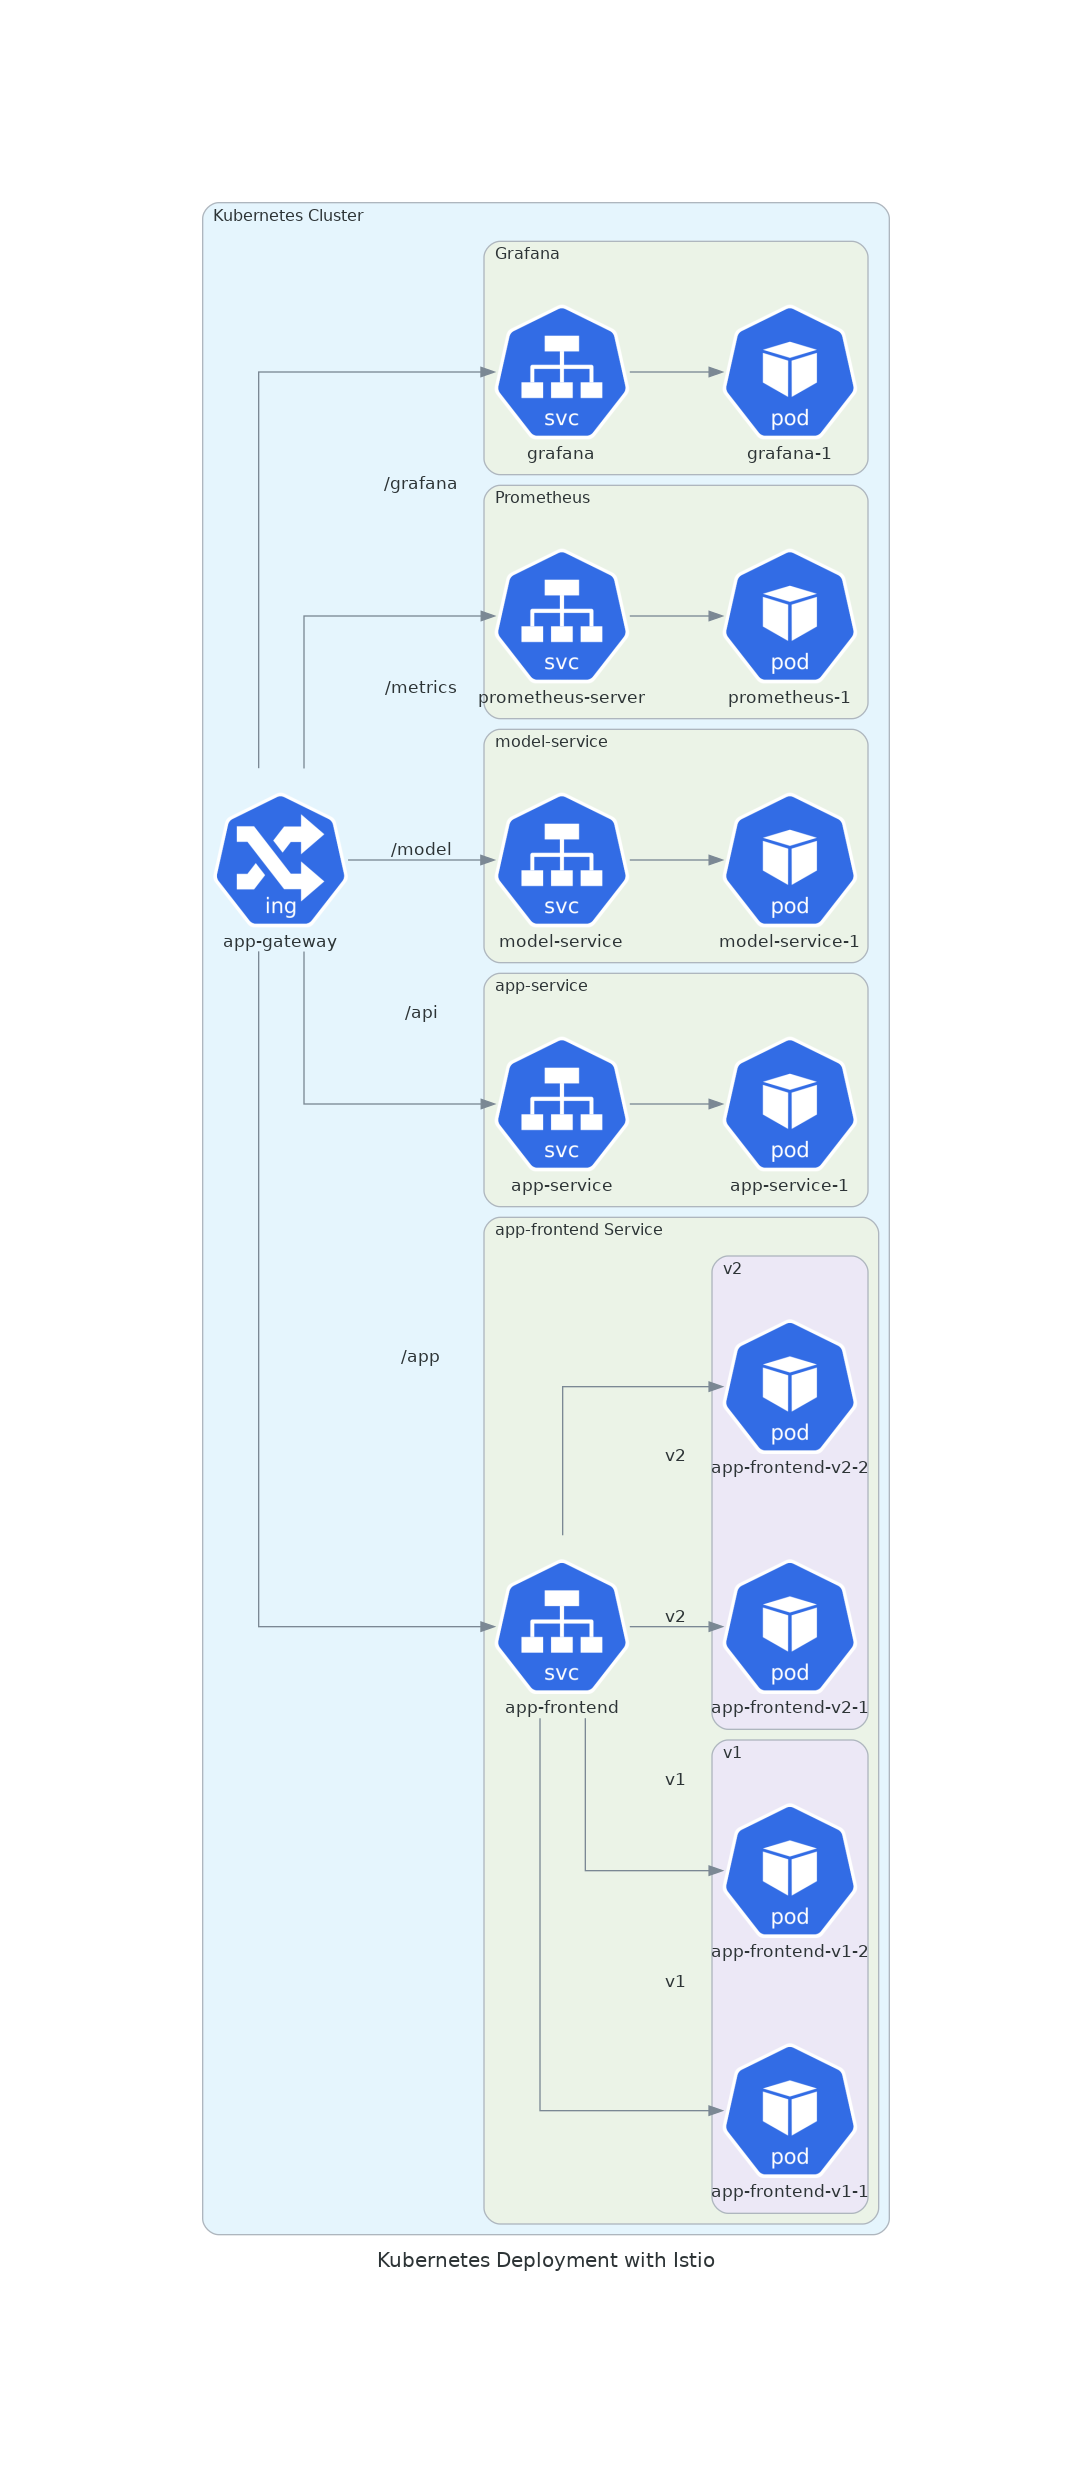
\includegraphics[width=\linewidth]{kubernetes_deployment_with_istio.png}
    \caption{Diagram of Kubernetes Deployment with Istio Gateway and Virtual Services}
    \label{fig:k8s_istio}
\end{figure}



% Insufficient -> The extension is unrelated to the release engineering practices and focuses on an implementation aspect. The extension is trivial or irrelevant for the current project.
% Sufficient -> The report describes a meaningful extension to either the training pipeline, release pipeline, contribution process, or deployment. It does not have to cover more than one.
% Good -> The report contains a critical reflection on the existing design and provides a convincing argumentation of a current shortcoming and its negative effect.
% Very Good -> The presented solution is clearly addressing the described shortcoming. The report also includes a brief explanation of how the success could be measured objectively.
% Excellent -> The presented extension is general in nature. It is relevant and applicable beyond the context of the concrete project.

\section{Project State}
As is only natural, no project is only smooth sailing. Every design decision has its risks and pitfalls. In this section we therefore reflect on the current state of the project, discuss what went wrong and how to improve.
\subsection{Limitations}
% Critically reflect on the current state of your project and identify the point that you find the most critical/annoying/error prone. Equipped with the knowledge of the course.
% Describe the identified shortcoming and its effect. A convincing argumentation is crucial.
During development the biggest pitfall was definitely the Kubernetes provisioning. After many failed attempts trying minikube or k3d, finally k3s ended up working.

Furthermore, a limitation, which we have also previously mentioned is that fact that we have secrets in our docker images. We currently have this way of handling things to allow public access to the repository. In general, if we had restricted access to the application, we would probably have to instruct people how to change a configuration file with some credentials in order to get the system to work. Alternatively, we could maintain the current way of doing things, but add a step where we encrypt the secrets and decrypt them with a key we would provide to intended users.

This a development-related limitation, but right now, every time we update an image, the entire packages and libraries have to be downloaded. This is especially problematic for \texttt{model-service} as it's dependencies are around 1.5GB. We can instead cache the libraries and use docker to check whether there is a library cache on the machine and whether the versions of the dependencies match with the ones specified in the pipenv/poetry file. This would improve the download time of the image.

Another limitation however, is the way we store the machine learning model. Right now we use DVC Live to pull the model. This has the disadvantage of needing access to the DVC GitHub repository in order to get the model. It also requires having access to secrets in order to access the storage where DVC data is stored. This is a lot of unnecessary overhead, considering model-service only needs to download a copy of the model, which created a lot of problems during it's implementation.   

Focusing more on release engineering practices we notice the system's monitoring and experimentation capabilities are fairly limited. We do collect some useful metrics, such as the number of active requests, the total number of requests with corresponding histograms. However, in order to monitor the model itself more complex steps must be taken. \\
Regarding the experimentation, our pipeline does support multiple releases which we can use for A/B testing. However, this can be extended to support gradual rollouts. We have to provide additional configurations to Istio in order to support this.   

\subsection{Extension} % or refactoring
% • Describe and visualize a project refactoring/extension that improves the situation.
% • Link to information sources that provide useful information about the problem, inspiration for your solution, or concrete examples for its realization. We expect that you cite respectable sources (e.g., research papers; quality blogs like Medium; tool websites; or popular StackOverflow discussions).
% • Describe how you could test whether the changed design would solve the original shortcoming.
To mitigate the problem described in the previous section, we can migrate from using DVC live to and AWS s3 bucket. We can see the difference in the two approaches in Figure {\color{red}\ref{fig:fetch-model-workflows}}. The main advantage is that we no longer would need a secret to access the model, making the application more secure, since we wouldn't have to deal with the problem of secrets being stored in files as previously mentioned. The logic of uploading the model would be moved to the \texttt{model-training} component. We would know this would solve the initial problem, since no more secrets would be stored in images and also would create a more pronounced isolation layer between \texttt{model-service} and \texttt{model-training}. \\

Additionally, to improve ML monitoring, concept drift detection would be a great improvement. Currently, we can automatically train a model and deploy it. However, apart from the metrics we collect during training, we do not know how the model is performing over time, due to changes in data for example. A concept drift detector can solve this problem by monitoring the error rate of a model or the changes in the distribution of the data over time.  
. 

\begin{figure*}[h]
    \centering
    \begin{subfigure}[b]{0.45\linewidth}
        \centering
        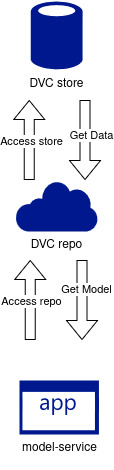
\includegraphics[width=0.35\linewidth]{images/original_fetch.jpg}
        \caption{Visualization of original workflows for fetching the model}
        \label{fig:libversion-workflow1}
    \end{subfigure}
    \hfill
    \begin{subfigure}[b]{0.45\linewidth}
        \centering
        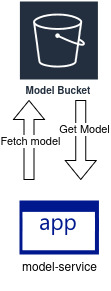
\includegraphics[width=0.35\linewidth]{images/improved_fetch.jpg}
        \caption{Visualization of improved workflow for fetching the model}
        \label{fig:libversion-workflow2}
    \end{subfigure}
    \caption{Side by side visualizations of \texttt{lib-version} workflows}
    \label{fig:fetch-model-workflows}
\end{figure*}

\section{Istio}
TODO

\subsection{Rate Limiting} % replace if we decide to implement another use case
% • General description of the use case.
% • The changes compared to the base design in the Deployment section.
TODO

\subsection{Experimental Setup}
% • General description of the experiment.
% • The changes compared to the base design in the Deployment section.
% • The hypothesis that is tested in the experiment.
% • The relevant metrics, i.e., what is being measured and how this is achieved.
% • A description of the decision process. More concretely, which data will be available (e.g., a Grafana screenshot) and how it will be used to derive a decision/answer regarding the hypothesis.
TODO
% As part of the assignment on ML Config Management, you had to configure your training pipeline
% using best practices and tools. Document how your pipeline is set up and the decisions you had to make to configure your project (tools, design, workarounds, and so on). This should come along with a description of your pipeline, its different steps, the tasks you have automated, which artefacts are being created, and so on.

\section{ML Pipeline}
As described previously, the aim of the \texttt{model-training} repository is to automate the process of training and publishing the model. However, setting up Continuous Integration, Continuous Delivery and Continuous Deployment proves to be more challenging than for regular software applications. 

\subsection{Configuration Tools}
For this reason additional configuration tools are required. For example, how can we perform version control for datasets and models? Or how can we detect code smells specific to Machine Learning code?
In order to solve these problems we make use of the tools:

\subsubsection{Poetry:}
Often repositories contain a \texttt{requirements.txt} as a method of managing dependencies. However, there is still a possibility that different collaborators are using different versions of the dependencies. {\color{blue} \href{https://python-poetry.org/}{Poetry}} is a tool which can sole this issue. It resolves dependencies before installation using a lock file to ensure compatibility across different environments. Another advantage of Poetry is the direct integration of virtual environment management. This will reduce the number of steps in the workflow. \\
Initially, we used {\color{blue} \href{https://pipenv.pypa.io/en/latest/}{Pipenv}} instead of Poetry for dependency management, however, we had issues with the Pipenv virtual environment when setting up the pipeline. For this reason we decided to switch.

\subsubsection{DVC:} \label{sec:ml-pipeline:dvc}
It is inconvenient to store large files directly in a Repository. To solve this, we use {\color{blue} \href{https://dvc.org/}{DVC}} to track large file such as datasets and models instead of Git. DVC's integration with Google Drive allows us to store these large files there. Additionally, this feature allows us to track changes to datasets and revert to previous versions if necessary. \\
Another advantage of DVC is the pipeline management. We can define stages in the project's workflow, such as data preprocessing, training, and evaluation. DVC automates the workflow by detecting changes and re-running only the impacted stages.

\subsubsection{Pylint \& dslinter:} \label{sec:ml-pipeline:lint}
Another problem of Machine Learning applications is code quality. As stated by Zhang et al. \cite{zhang2022code} "There is a lack of guidelines for code quality in machine learning applications. In particular, code smells have rarely been studied in this domain".
Therefore, we configure a linter to detect the code smells identified by Zhang et al. \\
As a basis, {\color{blue} \href{https://pylint.pycqa.org/en/latest/index.html}{Pylint}} serves as a linter for regular Python projects. We add a {\color{blue} \href{https://github.com/remla24-team12/model-training/blob/main/.pylintrc}{.pylintrc}} file in which we can configure custom rules. For a proper Machine Learning configuration we use {\color{blue} \href{https://github.com/SERG-Delft/dslinter}{dslinter}}. This is a Pylint plugin which helps ensure code quality specifically for Machine Learning. Dslinter provides a {\color{blue} \href{https://github.com/SERG-Delft/dslinter/blob/main/docs/pylint-configuration-examples/pylintrc-for-ml-projects/.pylintrc}{.pylintrc}}, which we used a basis. \\
% TODO: Explain why we didn't use any of the other linters: flake8, Bandit, etc.


\subsubsection{Pytest:}
In order to test different aspects of the model, we use {\color{blue} \href{https://pytest.org}{Pytest}} to create test suites. Please see the following section for more information about testing.

\subsection{Workflow}


\begin{figure*}
    \centering
    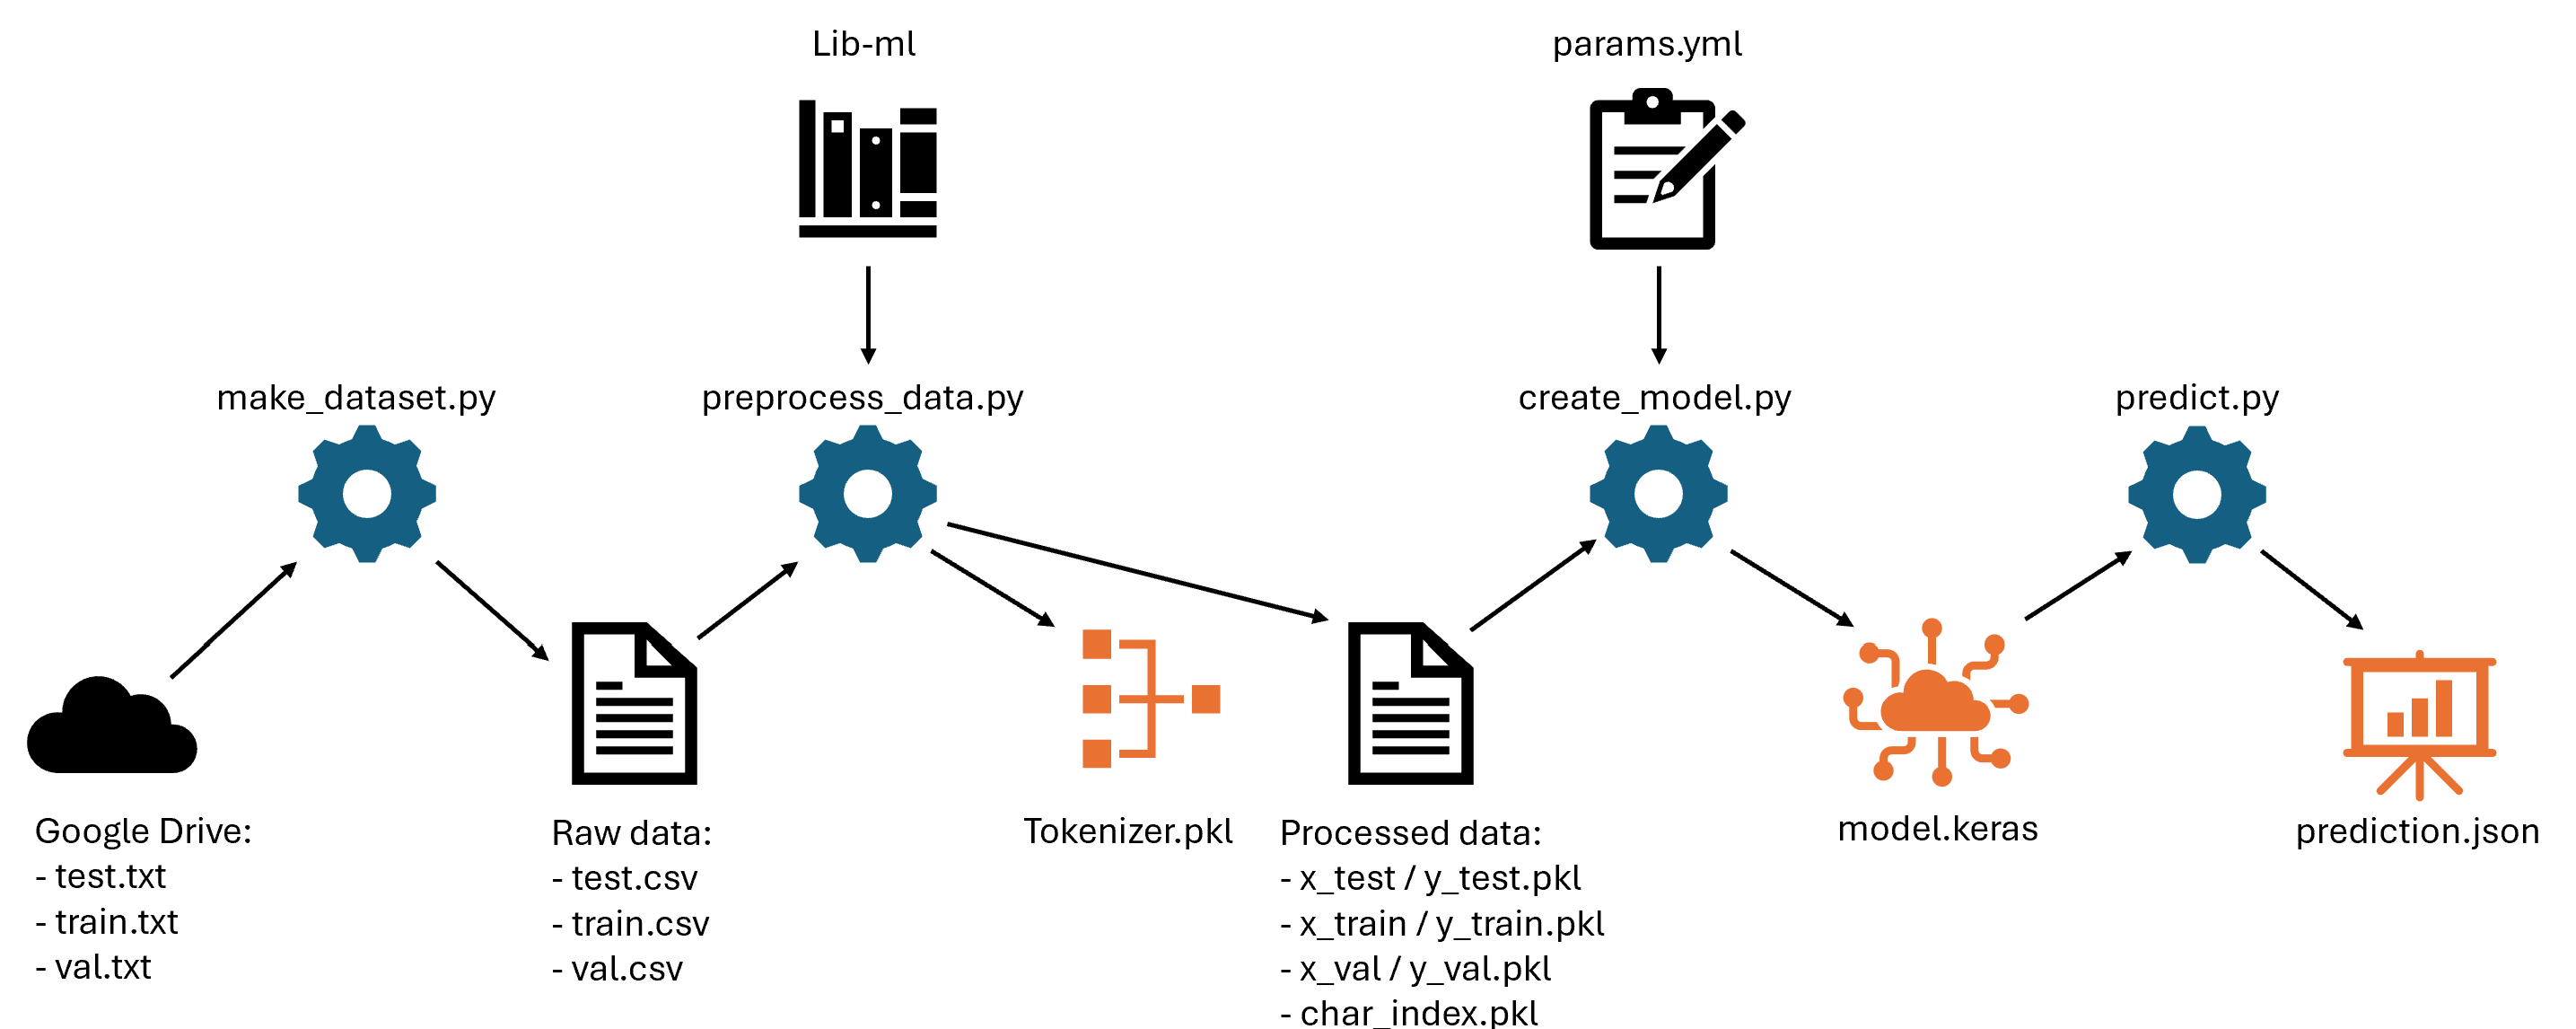
\includegraphics[width=0.75\linewidth]{images/ml_pipeline.png}
    \caption{Machine Learning Pipeline (orange = artifact)}
    \label{fig:ml-pipeline}
\end{figure*}
% As part of the assignment on ML Testing, you had to design a testing strategy and implement
% some automated tests. In this section, we expect you to fully document your choices and to reflect on limitations of the existing testing strategy. Moreover, we would like to hear your thoughts on how to improve tests, which new tests should be implemented and why.

\section{ML Testing Design}
In order to verify our entire systems functions correctly, reliably and effectively, we have set up an extensive Continuous Integration (CI) pipeline. The following subsections will elaborate on the testing and benchmark steps, test adequacy metrics and future improvements.

\subsection{Test Strategy}
Our testing strategy was guided by the paper \textit{What’s your ML Test Score? A rubric for ML production systems} \cite{mltestscore}. Four main aspects of ML testing are outlined, as well as a system of computing an ML test score. We have implemented the following tests based on these aspects:

\subsubsection{Tests for Features and Data:} Since the behaviour of ML systems learned from data, it is important to verify that the data delivered and handled as expected. We have implemented tests to verify that all steps in the DVC pipeline create correct output files. Additionally, the input features are checked for duplicate data.

\subsubsection{Tests for Model Development:} This testing aspect is not covered by explicit tests, but by how we have set up our testing suite. The paper recommends testing against a much simpler model as a baseline so the functionality of the whole pipeline can be quickly confirmed. Section \ref{sec:ml-tests:pipeline} elaborates more on this.

\subsubsection{Tests for ML Infrastructure:} To test the ML infrastructure, we are testing the reproducibility of training the model. The model is trained two times on the same data, but with different seeds. We can detect non-determinism when the accuracy of these models differs more than a threshold.

\subsubsection{Monitoring Tests for ML:} To monitor how our ML pipeline performs, we have implemented a benchmark using 
{\color{blue} \href{https://pypi.org/project/pytest-benchmark/}{PyTest Benchmark}}. Paired with the GitHub Action {\color{blue} \href{https://github.com/benchmark-action/github-action-benchmark/tree/master}{github-action-benchmark}}, the performance of training the model is automatically measured and compared to previous runs. If the change is too drastic, the pipeline will raise an error.

\subsection{Test Adequacy}
As highlighted by Zhang et al. \cite{zhang2019machine} a proper ML testing strategy covers a lot more aspects than the test score. As such, another important 'angle' is adequacy: "Test adequacy criteria are used to provide quantitative measurement on the degree of the target software that has been tested." \cite{zhang2019machine}. \\
The first criterion described in the same paper is neuron coverage. This metric is computed as the number of unique neurons activated by all test inputs over the total number of neurons in a network. The resulting percentage can provide useful insight about the training strategy of the model, as a low score indicates many neurons in the network are not contribution and may be pruned for example.
For our {\color{blue} \href{https://github.com/remla24-team12/model-training/blob/main/tests/adequacy/test_neuron_coverage.py}{implementation}} the number of neurons is determined by the convolutional and feed forward layers.

\subsection{Improvements}
A single adequacy metric alone is quite limited for a thorough adequacy report. In our view, by implementing the neuron coverage we created a solid foundation to which more adequacy criteria should be added in the future.  \\
Furthermore, we did not implement mutamorphic testing to further test the robustness and reliability of our model. We can create mutations of data samples, now if the test between these mutations and the original samples is very different, we know we have to make changes to the model to improve its robustness. Additionally, we can use mutations to repair inconsistencies in the data. \\
Finally we want to add tests more tests regarding for example irrelevance of the model. Meaning that it should ignore parts of the URL which are less relevant such as the 'http(s)://' sequence. Another test case is the impacts of hyperparameters. Parameters like the dropout ratio and learning rate (which is set to default 0.001) are currently hard-coded. Firstly, we should make them variable. Afterwards, we want to experiment with different values, in order to measure their impact.


\bibliographystyle{ACM-Reference-Format}
\bibliography{references}

\end{document}
\endinput
